\section{What is a Matrix}

A matrix is basically a notation convention that enables us to do some stuff more easily with a pencil and paper.  A very similar concept to this is the long division algorithm for for dividing two integers. For example consider the following long division (in French-European style) that we are all familiar with

\begin{equation*}
	\opdiv[decimalsepsymbol={,},displayintermediary=all,voperation=top]
	{198}{12}
\end{equation*}

So this notation and algorithms is to use some calculations more continent when is done by hand with a pen and paper. So the matrix notation can also be though as a computation convention. To make stuff more clear, consider the following example. \newline

\begin{example}{Simple Pen and Paper Calculations}
	Consider $V$ which is written as:
	\[ V = 2A + 3B + 4C \]
	
	Given the following relation between $A,B$, and $C$, rewrite $V$ in terms of $x,y$, and $z$.
	\begin{align*}
		A &= x + 2 y + 3 z \\
		B &= 2 x - y + z \\
		C &= -x -y + z
	\end{align*}
	
	\emph{Solution 1.}
	
	To write $V$ in terms of $x,y$, and $z$ we write:
	\begin{equation}
		V = 2 (x + 2 y + 3 z) + 3 (2 x - y + z) + 4 (-x -y + z)
		\label{example:SimplePenPaper:expandedForm}
	\end{equation}
	
	By arranging the terms using simple algebra we will have:
	
	\begin{equation}
		V = (2+6-4)x + (4-3-4)y + (6+3+4)z  = 4x -3y + 13z
		\label{example:SimplePenPaper:expanded2}
	\end{equation}


	\emph{Solution 2.}
	
	The calculations described in the first solution are not systematic. What I mean is that we started doing whatever we can do with you thinking about doing it in a more smart way that can also by systematically scaled to larger equations. This is where the matrices come into play. Matrices help us to do such calculations in a more algorithmic way (like the long division notation in which we do the calculations in a algorithmic way). \newline
	
	Let $\mathbb{B}$ be the set of all \emph{objects} that the $V$ is expanded in terms of and call this set as the \emph{basis} set. So for $\vect{V}= 2A + 3B + 4C$ we have the basis
	\[ \mathbb{B}_1 = \{ A,B,C \}. \]
	We can arrange the coefficients of $V$ in basis $\mathbb{B}_1$ in the following way:
	\begin{equation*}
		V_{\mathbb{B}_1}=
		\begin{pmatrix}
			2 \\
			3 \\
			4
		\end{pmatrix}_{\mathbb{B}_1}
	\end{equation*}
	We call it the coordinates of $V$ in the basis $\mathbb{B}_1$. Since we want to write the vector $V$ in terms of $x,y$, and $z$, we need to introduce the new basis $\mathbb{B}_2$ in the following way:
	
	\begin{equation*}
		\mathbb{B}_2 = \{ x,y,z \}
	\end{equation*}
	
	 Since $A,B$, and $C$ are expressed in terms of $x,y$, and $z$, we can arrange the coordinates of $A,B$, and $C$ in the basis $\mathbb{B}_2$ in the following way:
	 
	 \begin{equation*}
	 	L_{\mathbb{B}_1}^{\mathbb{B}_2} = \begin{pmatrix}
	 		1 & 2 & -1 \\
	 		2 & -1 & -1 \\
	 		3 & 1 & 1
	 	\end{pmatrix}_{\mathbb{B}_1}^{\mathbb{B}_2}
	 \end{equation*}
 
 	in which every column is the coefficients $A,B$, and $C$ in the basis $\mathbb{B}_2$ respectively. Note the subscript and the superscripts of the matrix. This matrix means that its columns contains the coordinates of the basis $\mathbb{B}_1$ in the new basis $\mathbb{B}_2$. So when it is applied to any vector that is described in basis $\mathbb{B}_1$, we will get the components of that vector in the basis $\mathbb{B}_2$. In other words:
 	
 	\begin{equation*}
 		V_{\mathbb{B}_2} = L_{\mathbb{B}_1}^{\mathbb{B}_2} V_{\mathbb{B}_1}
 	\end{equation*}
 
	\begin{equation}
		V_{\mathbb{B}_2} = 
		\begin{pmatrix}
			1 & 2 & -1 \\
			2 & -1 & -1 \\
			3 & 1 & 1
		\end{pmatrix}_{\mathbb{B}_1}^{\mathbb{B}_2}
		\begin{pmatrix}
			2 \\
			3 \\
			4
		\end{pmatrix}_{\mathbb{B}_1}
		\label{example:SomplePenPaper:matrixEquation}
	\end{equation}

	Considering the basic operations introduced with matrix notation, this matrix equation can be written in two ways as described below:
	
	\begin{equation}
		V_{\mathbb{B}_2} = 
		2 \begin{pmatrix}
			1 \\
			2 \\
			3
		\end{pmatrix}_{\mathbb{B}_2} 
		+ 3 \begin{pmatrix}
			2 \\
			-1 \\
			1
		\end{pmatrix}_{\mathbb{B}_2}
		+ 4 \begin{pmatrix}
			-1 \\
			-1 \\
			1
		\end{pmatrix}_{\mathbb{B}_2}
	\end{equation}

	The equation above is equivalent to equation \ref{example:SimplePenPaper:expandedForm} but described in other way! Also the other way to write the matrix equation \ref{example:SomplePenPaper:matrixEquation} is the following way in which we have used the matrix multiplication conventions:
	
	\begin{equation}
		V_{\mathbb{B}_2} = 
		\begin{pmatrix}
			1 & 2 & -1 \\
			2 & -1 & -1 \\
			3 & 1 & 1
		\end{pmatrix}_{\mathbb{B}_1}^{\mathbb{B}_2}
		\begin{pmatrix}
			2 \\
			3 \\
			4
		\end{pmatrix}_{\mathbb{B}_1}
		=\begin{pmatrix}
			(1*2) + (2*3) + (-1*4) \\
			(2*2) + (-1*3) + (-1*4) \\
			(3*2) + (1*3) + (1*4))
		\end{pmatrix}_{\mathbb{B}_2}	
		=\begin{pmatrix}
			4 \\
			-3 \\
			13
		\end{pmatrix}_{\mathbb{B}_2}		
	\end{equation}

	which is essentially equivalent to the equation \ref{example:SimplePenPaper:expanded2} but written in a different way.
	
	 
\end{example}

\section{Linear Operators and Matrices}

Consider the vector spaces $ \vectSpace{V}  $ and $ \vectSpace{W} $ by are spanned with $ \basis{B}{\vectSpace{V}}{a}{i}{N} $ and $ \basis{B}{\vectSpace{W}}{b}{j}{M} $ respectively. The act of a linear operator $ A \in \vectSpace{L}(\vectSpace{V},\vectSpace{W}) $ on the vector $ \ket{v} \in \vectSpace{V} $ can be specified by its act on the basis of that vector space $ \mathbb{B}_\vectSpace{V} $. Suppose that $ A $ acts on the basis vectors $ \ket{a_i} $ as the following:

\begin{equation}
	\begin{split}
		\ket{w_i} = A \ket{a_i} = \sum_{j=1}^{M} \rho_{ji} \ket{b_j}
	\end{split}
\end{equation}

in which $ \rho_{ji} $ are the components of $ \ket{w_i} $ in the basis $ \mathbb{B}_\vectSpace{W} $ and can be organized as column vectors:

\begin{equation*}
	\underline{w_i}_{\mathbb{B}_\vectSpace{W}} = \begin{pmatrix}
		\rho_{1i} \\
		\rho_{2i} \\
		\vdots \\
		\rho_{Mi}
	\end{pmatrix}_{\mathbb{B}_\vectSpace{W}}
\end{equation*}

Now if $ A $ acts on the vector $ \ket{v} = \sum_{i=1}^{N} \alpha_i \ket{a_i} $ can be written as:

\begin{equation*}
	\ket{u} = A\ket{v} = A\sum_{i=1}^{N} \alpha_i \ket{a_i} = \sum_{i=1}^{N} \alpha_i A\ket{a_i} = \sum_{i=1}^{N} \alpha_i \sum_{j=1}^{M} \rho_{ji} \ket{b_j} =  \sum_{j=1}^{M} \underbrace{\sum_{i=1}^{N} \alpha_i \rho_{ji}}_{\eta_j}\ket{b_j} = \sum_{j=1}^{M} \eta_j \ket{b_j}
\end{equation*}

so the coordinates of the vector $ \ket{u} = A \ket{v} $ will be:

\begin{equation}
	\eta_j = \sum_{i=1}^{N} \alpha_i \rho_{ji}
	\label{equ:LLinearOperatorAndMatrix:newComponents}
\end{equation}

which also can be written as:

\begin{equation*}
	\underline{u}_{\mathbb{B}_\vectSpace{W}} = \begin{pmatrix}
		\eta_1 \\
		\eta_2 \\
		\vdots \\
		\eta_j
	\end{pmatrix}_{\mathbb{B}_\vectSpace{W}}
\end{equation*}


The above equation is very important and can be shown in matrix notation to make the idea more clear. To do this we need to build matrix $ \mat{A}_{\mathbb{B}_\vectSpace{V}}^{\mathbb{B}_\vectSpace{W}} $ by arranging the components of $\underline{w_i}_{\mathbb{B}_\vect{W}}$ as the columns of $ \mat{A}_{\mathbb{B}_\vectSpace{V}}^{\mathbb{B}_\vectSpace{W}} $:

\begin{equation}
	\mat{A}_{\mathbb{B}_\vectSpace{V}}^{\mathbb{B}_\vectSpace{W}} = \begin{pmatrix}
		\rho_{11} & \rho_{12} & \cdots & \rho_{1N}\\
		\rho_{21} & \rho_{22} & \cdots & \rho_{2N}\\
		\vdots    & \vdots    & \ddots & \vdots\\
		\rho_{M1} & \rho_{M2} & \cdots & \rho_{MN} 
	\end{pmatrix}_{\mathbb{B}_{\vectSpace{V}}}^{\mathbb{B}_\vectSpace{W}}
\end{equation}

So the equation \ref{equ:LLinearOperatorAndMatrix:newComponents} can be written as:

\begin{LARGE}
	\begin{equation}
		\boxed{
		\underline{u}_{\mathbb{B}_\vectSpace{W}} = \mat{A}_{\mathbb{B}_\vectSpace{V}}^{\mathbb{B}_\vectSpace{W}} \underline{v}_{\mathbb{B}_\vectSpace{V}}
		}
	\end{equation}
	\label{equ:matrixAndLinearOperator_compact}
\end{LARGE}


Note that a matrix does not have any meaning by itself and is just a collection of numbers. To correspond any matrix with a linear operator $ A \in \vectSpace{L}(\vectSpace{V},\vectSpace{W})$, we need to fix the basis vectors $ \mathbb{B}_{\vectSpace{V}} $ and $ \mathbb{B}_{\vectSpace{W}} $.






\section{Change of Basis}

As we discussed earlier, the matrix representation of a linear operator $\op{A} \in \vectSpace{L}(\vectSpace{V},\vectSpace{W})$ depends on the choice of basis $\mathbb{B}_{\vectSpace{V}}$ and $\mathbb{B}_\vectSpace{W}$ which are the basis of vector spaces $\vectSpace{V}$ and $ \vectSpace{W} $ respectively. Now suppose that that in the vector spaces $\vectSpace{V}$, the elements are described in basis $\mathbb{B}_1 = \{ \ket{e_i} \}_{i=1}^{N}$ but we want to change it to the basis $\basis{B}{2}{e'}{j}{N}$. We need to know the relation between these two basis that is assumed to be the following:

\begin{equation}
	\ket{e_i} = \sum_{j=1}^{N} \rho_{ji} \ket{e'_{j}}
	\label{equ:changeOfMatrix:eInTermsOfePrime}
\end{equation}

Consider the vector $\ket{v}$ that is described in the basis $\mathbb{B}_1$ in the following way: 

\begin{equation}
	\ket{v} = \sum_{i=1}^{N} \alpha_i \ket{e_i} 
	\label{equ:changeOfBasis:expansionOfvIne}
\end{equation}

\[ \ket{v} = \sum_{i=1}^{N} \alpha_i \ket{e_i} \] 

The coefficients of the expansion are called the \emph{coordinates} of $\ket{v}$ in the basis $\mathbb{B}_1$ and can be shown like:

\begin{equation}
	\underline{v}_{\mathbb{B}_1} = \begin{pmatrix}
		\alpha_1 \\
		\alpha_2 \\
		\vdots \\
		\alpha_N
	\end{pmatrix}_{\mathbb{B}_1}
\end{equation}

Now we can use the equation \ref{equ:changeOfMatrix:eInTermsOfePrime} to replace $\ket{e_i}$ in \ref{equ:changeOfBasis:expansionOfvIne} with $\ket{e'_j}$:

\begin{equation}
	\ket{v} = \sum_{i=1}^{N} \sum_{j=1}^{N}\alpha_i \rho_{ji} \ket{e'_j} = \sum_{j=1}^{N} \sum_{i=1}^{N}\rho_{ji} \alpha_i  \ket{e'_j}  = \sum_{j=1}^{N} \eta_j \ket{e'_j}
	\label{equ:chanbeOfBasis:vInNewBasis}
\end{equation}

in which $\eta_j = \sum_{i=1}^{N}\rho_{ji} \alpha_i $ is the coordinates of $ \ket{v} $ in the new basis $\mathbb{B}_2$:

\begin{equation*}
	\underline{v}_{\mathbb{B}_2} = \begin{pmatrix}
		\eta_1 \\
		\eta_2 \\
		\vdots \\
		\eta_N
	\end{pmatrix}_{\mathbb{B}_2}
\end{equation*}


The equation \ref{equ:chanbeOfBasis:vInNewBasis} can be written in the following matrix equation:

\begin{equation}
	\begin{pmatrix}
		\eta_1 \\
		\eta_2 \\
		\vdots \\
		\eta_N
	\end{pmatrix}_{\mathbb{B}_2} = 
	\underbrace{\begin{pmatrix}
			\rho_{11} & \rho_{12} & \cdots & \rho_{1N}\\
			\rho_{21} & \rho_{22} & \cdots & \rho_{2N}\\
			\vdots    & \vdots    & \ddots & \vdots\\
			\rho_{N1} & \rho_{N2} & \cdots & \rho_{NN} 
		\end{pmatrix}_{\mathbb{B}_1}^{\mathbb{B}_2}}_{R}
	\begin{pmatrix}
		\alpha_1 \\
		\alpha_2 \\
		\vdots \\
		\alpha_N
	\end{pmatrix}_{\mathbb{B}_1} 
\end{equation}

That can also be written in a more compact form:

\begin{LARGE}
	\begin{equation}
		\boxed{
			\underline{v}_{\mathbb{B}_2} = \mat{R}_{\mathbb{B}_1}^{\mathbb{B}_2} \underline{v}_{\mathbb{B}_1}
		}
	\end{equation}
	\label{equ:changeOfBasis_compact}
\end{LARGE}

The matrix $R$ is called the change of basis matrix. \newline

\begin{example}{Change of Basis}
	Consider the following Cartesian plane:
	
\begin{center}
	\tikzset{every picture/.style={line width=0.75pt}} %set default line width to 0.75pt        
	
	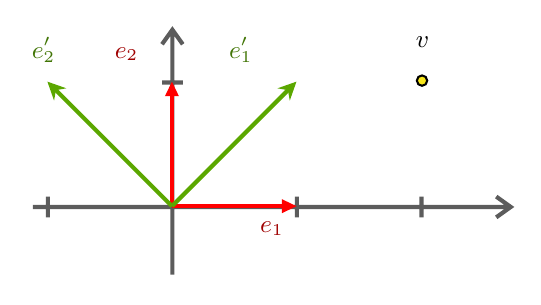
\begin{tikzpicture}[x=0.75pt,y=0.75pt,yscale=-1,xscale=1]
		%uncomment if require: \path (0,300); %set diagram left start at 0, and has height of 300
		
		%Shape: Axis 2D [id:dp342570794536994] 
		\draw [color={rgb, 255:red, 92; green, 92; blue, 92 }  ,draw opacity=1 ][line width=1.5]  (113,200.38) -- (343.25,200.38)(180.22,115) -- (180.22,233) (336.25,195.38) -- (343.25,200.38) -- (336.25,205.38) (175.22,122) -- (180.22,115) -- (185.22,122) (240.22,195.38) -- (240.22,205.38)(300.22,195.38) -- (300.22,205.38)(120.22,195.38) -- (120.22,205.38)(175.22,140.38) -- (185.22,140.38) ;
		\draw   ;
		%Straight Lines [id:da1818651961566673] 
		\draw [color={rgb, 255:red, 255; green, 0; blue, 0 }  ,draw opacity=1 ][line width=1.5]    (180,200) -- (236,200) ;
		\draw [shift={(240,200)}, rotate = 180] [fill={rgb, 255:red, 255; green, 0; blue, 0 }  ,fill opacity=1 ][line width=0.08]  [draw opacity=0] (6.97,-3.35) -- (0,0) -- (6.97,3.35) -- cycle    ;
		%Straight Lines [id:da6840376030942996] 
		\draw [color={rgb, 255:red, 255; green, 0; blue, 0 }  ,draw opacity=1 ][line width=1.5]    (180,200) -- (180,144) ;
		\draw [shift={(180,140)}, rotate = 90] [fill={rgb, 255:red, 255; green, 0; blue, 0 }  ,fill opacity=1 ][line width=0.08]  [draw opacity=0] (6.97,-3.35) -- (0,0) -- (6.97,3.35) -- cycle    ;
		%Straight Lines [id:da23828819589743078] 
		\draw [color={rgb, 255:red, 91; green, 167; blue, 0 }  ,draw opacity=1 ][line width=1.5]    (180,200) -- (237.17,142.83) ;
		\draw [shift={(240,140)}, rotate = 135] [fill={rgb, 255:red, 91; green, 167; blue, 0 }  ,fill opacity=1 ][line width=0.08]  [draw opacity=0] (8.75,-4.2) -- (0,0) -- (8.75,4.2) -- (5.81,0) -- cycle    ;
		%Straight Lines [id:da644259291625594] 
		\draw [color={rgb, 255:red, 91; green, 167; blue, 0 }  ,draw opacity=1 ][line width=1.5]    (180,200) -- (122.83,142.83) ;
		\draw [shift={(120,140)}, rotate = 45] [fill={rgb, 255:red, 91; green, 167; blue, 0 }  ,fill opacity=1 ][line width=0.08]  [draw opacity=0] (8.75,-4.2) -- (0,0) -- (8.75,4.2) -- (5.81,0) -- cycle    ;
		%Shape: Circle [id:dp8467208402612376] 
		\draw  [color={rgb, 255:red, 0; green, 0; blue, 0 }  ,draw opacity=1 ][fill={rgb, 255:red, 248; green, 231; blue, 28 }  ,fill opacity=1 ] (298,139.5) .. controls (298,138.12) and (299.12,137) .. (300.5,137) .. controls (301.88,137) and (303,138.12) .. (303,139.5) .. controls (303,140.88) and (301.88,142) .. (300.5,142) .. controls (299.12,142) and (298,140.88) .. (298,139.5) -- cycle ;
		
		% Text Node
		\draw (296,117) node [anchor=north west][inner sep=0.75pt]  [font=\small] [align=left] {$\displaystyle \ket{v}$};
		% Text Node
		\draw (221,206) node [anchor=north west][inner sep=0.75pt]  [font=\small,color={rgb, 255:red, 159; green, 0; blue, 0 }  ,opacity=1 ] [align=left] {$\displaystyle \ket{e_{1}}$};
		% Text Node
		\draw  [draw opacity=0]  (148,118) -- (182,118) -- (182,143) -- (148,143) -- cycle  ;
		\draw (151,122) node [anchor=north west][inner sep=0.75pt]  [font=\small,color={rgb, 255:red, 159; green, 0; blue, 0 }  ,opacity=1 ] [align=left] {$\displaystyle \ket{e_{2}}$};
		% Text Node
		\draw (206,117) node [anchor=north west][inner sep=0.75pt]  [font=\small,color={rgb, 255:red, 65; green, 117; blue, 5 }  ,opacity=1 ] [align=left] {$\displaystyle \ket{e'_{1}}$};
		% Text Node
		\draw (111,117) node [anchor=north west][inner sep=0.75pt]  [font=\small,color={rgb, 255:red, 65; green, 117; blue, 5 }  ,opacity=1 ] [align=left] {$\displaystyle \ket{e'_{2}}$};
		
	\end{tikzpicture}


\end{center}

	
	The vectors of the plain can be expressed using any arbitrary basis two of which are provided here as an example:
	\begin{align*}
		\mathbb{B}_1 &= \{ \ket{e_1}, \ket{e_2} \} = \{ 
		\begin{pmatrix}
			1 \\
			0
		\end{pmatrix}_{\mathbb{B}_1},
		\begin{pmatrix}
			0 \\
			1
		\end{pmatrix}_{\mathbb{B}_1}
		\} \\
		\mathbb{B}_2 &= \{ \ket{e'_1}, \ket{e'_2} \} = \{ 
		\begin{pmatrix}
			1 \\
			0
		\end{pmatrix}_{\mathbb{B}_2},
		\begin{pmatrix}
			0 \\
			1
		\end{pmatrix}_{\mathbb{B}_2}
		\} = 
		\{ 
		\begin{pmatrix}
			1 \\
			1
		\end{pmatrix}_{\mathbb{B}_1},
		\begin{pmatrix}
			-1 \\
			1
		\end{pmatrix}_{\mathbb{B}_1}
		\}
	\end{align*}

	It is clear that the vector $ \ket{v} $ can be expanded like: 
	\begin{equation}
		\ket{v} = 2\ket{e_1} + \ket{e_2}
		\label{equ:changeOfBasis:example:v_in_terms_of_B1}
	\end{equation}
	
	So we can write:
	\[ \underline{v}_{\mathbb{B}_1} = \begin{pmatrix}
		2 \\
		1
	\end{pmatrix}_{\mathbb{B}_1} \]
	in which $\underline{v}_{\mathbb{B}_1}$ is the coordinates of $ \ket{v} $ in the basis $ \mathbb{B}_1 $. Now suppose that we want to fine the coordinates of $ \ket{v} $ in the basis $ \mathbb{B}_2 $. To do that we need to write the $ \ket{e_1} $ and $ \ket{e_2} $ in terms of  $ \ket{e'_1} $ and $ \ket{e'_2} $ (i.e. find the coordinates of elements of $ \mathbb{B}_1 $ in the basis $ \mathbb{B}_2 $):
	
	\begin{equation}
		\begin{split}
			\ket{e_1} &= \ket{e'_1} - \ket{e'_2} \\
			\ket{e_2} &= \ket{e'_1} + \ket{e'_2} 
		\end{split}
		\label{equ:changeOfBasis:example:B1_in_terms_of_B2}
	\end{equation}

	This can be written in the column vector format:
	\begin{align*}
		\underline{e_1}_{\mathbb{B}_2} &= \begin{pmatrix}
			1 \\
			-1
		\end{pmatrix}_{\mathbb{B}_2} , \quad
		\underline{e_1}_{\mathbb{B}_2} = \begin{pmatrix}
			1 \\
			1
		\end{pmatrix}_{\mathbb{B}_2}
	\end{align*}
	By arranging these columns into the columns of matrix we will get the change of basis matrix:
	\begin{equation*}
		\mat{R} = \begin{pmatrix}
			1 & 1 \\
			-1 & 1
		\end{pmatrix}_{\mathbb{B}_1}^{\mathbb{B}_2}
	\end{equation*}

	By inserting \ref{equ:changeOfBasis:example:B1_in_terms_of_B2} in \ref{equ:changeOfBasis:example:v_in_terms_of_B1} we can get the expanded form of $ \ket{v} $ in the new basis $\mathbb{B}_2$.
	
	\begin{equation*}
		\ket{v} = 2 (\ket{e'_1} - \ket{e'_2}) + (\ket{e'_1} + \ket{e'_2} ) = 3 \ket{e'_1} -\ket{e'_2} 
	\end{equation*}

	The above calculations can also be done by applying the change of basis matrix $ \mat{R} $ on the coordinates of $ \ket{v} $ in $ \mathbb{B}_1 $, i.e. $ \underline{v}_{\mathbb{B}_1} $ :
	\begin{equation*}
		\underline{v}_{\mathbb{B}_2} = \begin{pmatrix}
			1 & 1 \\
			-1 & 1
		\end{pmatrix}_{\mathbb{B}_1}^{\mathbb{B}_2}
		\begin{pmatrix}
			2 \\
			1
		\end{pmatrix}_{\mathbb{B}_1} = 
	\begin{pmatrix}
		3 \\
		-1
	\end{pmatrix}_{\mathbb{B}_2}
	\end{equation*}
\end{example}


The idea behind the change of basis matrix and the matrices corresponding to linear operator are very similar and this similarity can lead to confusions. For example the equations \ref{equ:matrixAndLinearOperator_compact} and \ref{equ:changeOfBasis_compact} are very similar but are very different at the same time. In the former case the vector $ \ket{v} $ changes to another vector $ \ket{w} $ but in the latter case the vector $\ket{v} $ remains unchanged and only gets represented with new coordinates in the new basis. So when we can know that a matrix changes the basis only and keeps the vector unchanged or maps the vector into another vector? The following example would clarify the differences.

\begin{example}{Linear Operators Matrices vs. Change of Basis Matrices}
	content..
\end{example}






